% Foto corregida del panel frontal con anotaciones
\begin{tikzpicture}[
  caja/.style={draw=#1,fill=white,fill opacity=.93,text opacity=1,rounded corners=1.5pt,
    font=\sffamily\scriptsize,inner sep=2.5pt,align=left,line width=.6pt},
  caja/.default=azul,
  flecha/.style={-{Stealth[length=4.5pt]},#1,line width=.8pt},
  flecha/.default=azul,
  num/.style={circle,fill=#1,text=white,font=\sffamily\bfseries\tiny,inner sep=0pt,
    minimum size=10pt,draw=white,line width=.5pt},
  num/.default=navy]
  \node[inner sep=0,anchor=south west] (img) at (0,0)
    {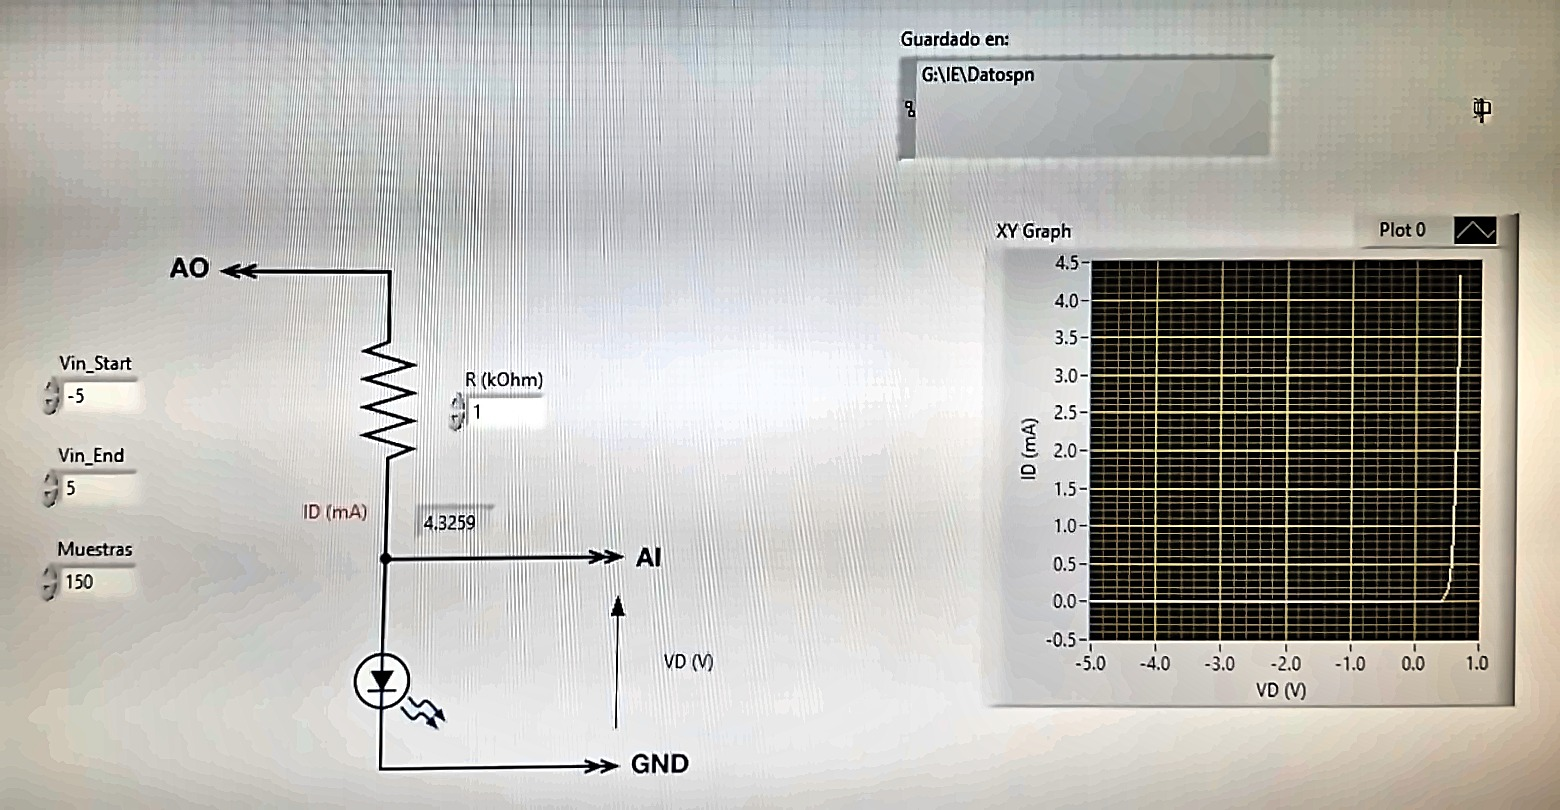
\includegraphics[width=\linewidth]{img/panel_frontal.jpg}};
  \begin{scope}[x={(img.south east)},y={(img.north west)}]
    % controles de la rampa
    \node[caja=ambar,anchor=west] (c) at (0.105,0.16)
      {\textbf{\textcolor{ambar}{\ding{172}} Controles numéricos (DBL)}\\
       rampa: $V_{\text{start}}=-5$\,V, $V_{\text{end}}=5$\,V,\\ 150 muestras};
    \draw[flecha=ambar] (c.north west) ++(0.012,0) -- (0.075,0.50);
    \draw[flecha=ambar] (c.north west) ++(0.022,0) -- (0.075,0.39);
    \draw[flecha=ambar] (c.west) -- (0.075,0.28);
    % R
    \node[caja=ambar,anchor=west] (r) at (0.36,0.62)
      {\textbf{\textcolor{ambar}{\ding{173}} Control $R$ (k$\Omega$)}\\ valor de la resistencia: 1};
    \draw[flecha=ambar] (r.west) -- (0.345,0.52);
    % indicador I_D
    \node[caja=cVerde,anchor=west] (i) at (0.455,0.43)
      {\textbf{\textcolor{cVerde}{\ding{174}} Indicador $I_D$ (mA)}\\ último valor: 4,326 mA\\ (con $V_{\text{in}}=5$\,V)};
    \draw[flecha=cVerde] (i.west) -- (0.335,0.37);
    % imagen del circuito
    \node[caja,anchor=north west] (img2) at (0.18,0.985)
      {\textbf{\textcolor{azul}{\ding{175}} Imagen importada (LED\_cir.png)}\\
       AO-0 impone $V_{\text{in}}$ sobre $R$ + diodo; AI-1 lee $V_D$;\\ GND es la masa común};
    \draw[flecha] (img2.south west) ++(0.03,0) -- (0.115,0.69);
    \draw[flecha] (img2.south) ++(0.02,0) -- (0.39,0.33);
    % ruta del fichero
    \node[caja=navy,anchor=east] (p) at (0.585,0.875)
      {\textbf{\textcolor{navy}{\ding{176}} Control de ruta}\\ fichero de salida (.txt)};
    \draw[flecha=navy] (p.east) -- (0.615,0.87);
    % gráfica XY
    \node[caja=cUV,anchor=east] (g) at (0.66,0.74)
      {\textbf{\textcolor{cUV}{\ding{177}} XY Graph}\\ eje $Y$: $I_D$ (mA)\\ eje $X$: $V_D$ (V)};
    \draw[flecha=cUV] (g.east) -- (0.74,0.66);
    % rama directa
    \node[caja=cUV,anchor=east] (k) at (0.905,0.56)
      {rama directa:\\ conduce a partir\\ de $V_u\approx0{,}6$\,V};
    \draw[flecha=cUV] (k.south east) ++(-0.005,0) -- (0.925,0.36);
    \node[caja=cUV,anchor=west] (corte) at (0.715,0.22)
      {corte: $I_D\simeq0$};
    \draw[flecha=cUV] (corte.north) -- (0.78,0.30);
  \end{scope}
\end{tikzpicture}
